\documentclass{beamer}

\newcommand{\zwischentitel}{Künstliche neuronale Netze}
\newcommand{\autor}{Florian Sihler}
\newcommand{\leitthema}{Clusteranalyse \& Klassifikation}
\newcommand{\titel}{Proseminar: Künstliche neuronale Netze}
\newcommand{\untertitel}{\leitthema}

\usetheme{lillyKIZ}

\begin{document}

    \begin{slide}{Das Ziel}
        \onslide<2-3>\begin{minipage}[t]{0.49\linewidth}
            \centering
            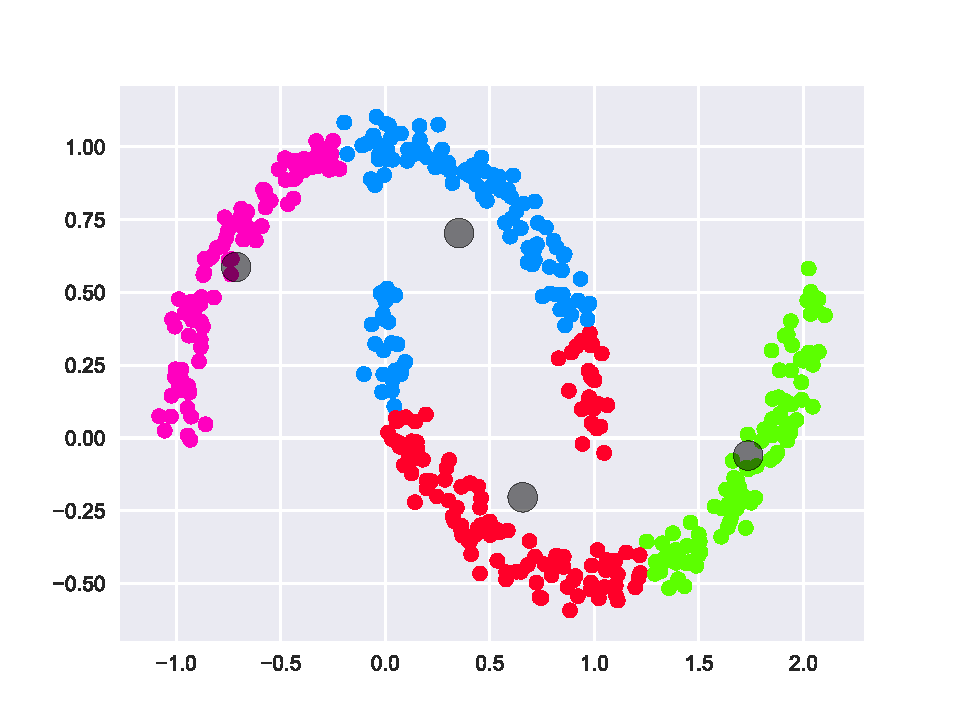
\includegraphics[width=\linewidth]{Data/4-km-moon.pdf}
            {\centering (a) ~k-Means\par}
        \end{minipage}
        \onslide<3>\begin{minipage}[t]{0.49\linewidth}
            \centering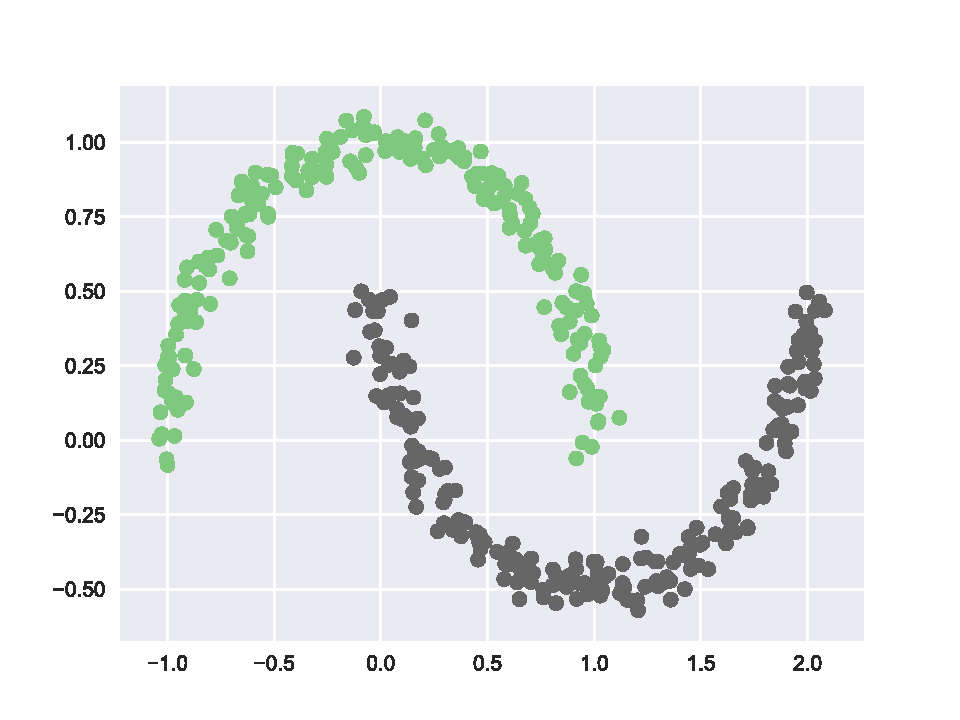
\includegraphics[width=\linewidth]{Data/42-knn-moon.pdf}
            {\centering (b) ~k-Nearest\par}
        \end{minipage}
    \end{slide}


    \begin{slide}{Behandelte Themen}
        \begin{bulletpoints}
            \pause\item \(k\)-Means
            \pause\item \(k\)-Nearest Neighbouring
            \pause\item \(\varepsilon\)-Nearest Neighbouring
            \pause\item ROLF - \textbf{R}egional and \textbf{O}nline \textbf{L}earnable \textbf{F}ields
        \end{bulletpoints}
    \end{slide}

\end{document}
